\section{SOMHunter Interface}
\label{sec:interface}

SOMHunter Tool has its user interface in the form web application. Thus you can use any modern browser to use it. Just visit the address where SOMHunter is running. In case you don't have that, ask your system administrator or visit developer documentation on how to build and launch the system.

After you open the beforementioned address, you should see the interface looking like \cref{fig:ui}.

\begin{figure}[h]
	\centering
	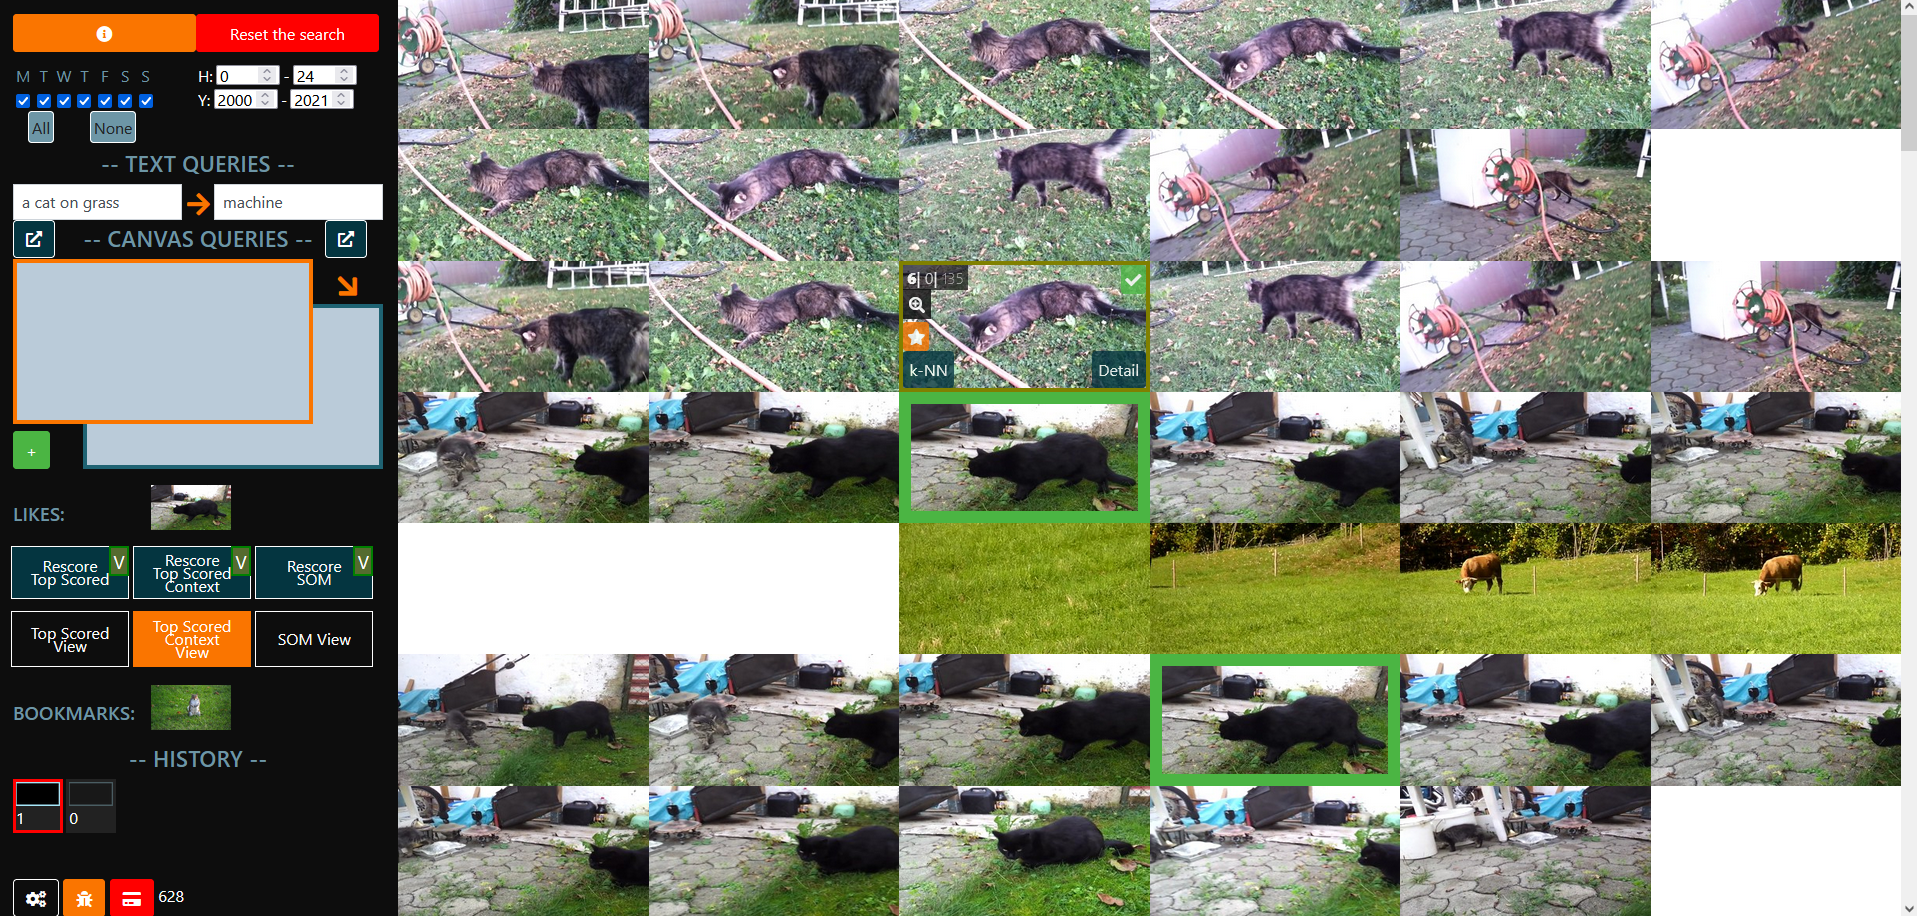
\includegraphics[width=1.0\textwidth]{img/ui.png}
  \caption{\textbf{SOMHunter Tool interface.}}
	\label{fig:ui}
\end{figure}


On the left side, there is the main panel, where you will construct the query and request rescores. The rest of the UI is current results displayed in a grid with the requested type of view (displays).  That is where you'll browse the results, provide the feedback by "liking" similar frames and look for the target scene(s).


%% %%%%%%%%%%%%%%%%%%%%%%%%%%%%%%%%%
\subsection{Textual Query}
\begin{figure}[h]
	\centering
	
\includegraphics[width=0.6\textwidth]{img/text-query.png}
  \caption{\textbf{Text querying interface panel.}}
	\label{fig:text-query}
\end{figure}

The textual querying is the most important part to formulate the query. There are two text inputs (see ~\cref{fig:text-query}) that allow you to formulate a so-called temporal query. That means that you are describing the two scenes that chronologically follow. For example, for the temporal query "A cat on a sofa" followed with "Dog barking at the door" we are describing part of the video with a scene where a cat is on a sofa followed with a scene of a barking dog.

As you can see, you can use natural language sentences to construct the queries. 


%% %%%%%%%%%%%%%%%%%%%%%%%%%%%%%%%%%
\subsection{Canvas Query}
\begin{figure}[h]
	\centering
  \begin{subfigure}[b]{0.5\textwidth}
      \centering
      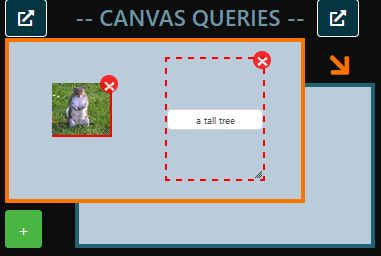
\includegraphics[width=\textwidth]{img/canvas-1.png}
      \caption{\textbf{Constructing the first canvas query.}}
  \end{subfigure}
  \hfill
  \begin{subfigure}[b]{0.5\textwidth}
      \centering
      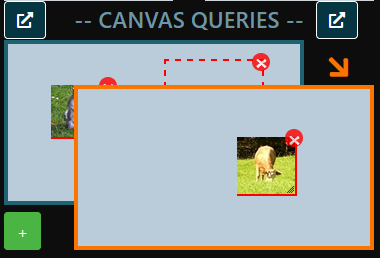
\includegraphics[width=\textwidth]{img/canvas-2.png}
      \caption{\textbf{Constructing the second canvas query.}}
  \end{subfigure}
	
  \caption{\textbf{Canvas querying interface panel}}
	\label{fig:canvas-query}
\end{figure}

The second option to formulate a temporal query is to use the canvases (see~\cref{fig:canvas-query}). With this, you have the advantage that you can specify approximate positions of the objects in the scene. Again the semantics of the temporality remains the same as in textual queries. Moreover, on a canvas, you can place both bitmaps and texts. 

To place a bitmap, just paste it from your clipboard by hitting Control+V (most GUIs of operating systems offer a keystroke to do create a rectangular snip from the screen directly to the clipboard; e.g. on Windows, it's Shift +Win + S). After that just reposition and scale it as you wish.

To place s text, hit the green plus button or do Shift + Left mouse click to the canvas. The textual input will appear. Just fill in the textual query, place and scale it as you require.

%% %%%%%%%%%%%%%%%%%%%%%%%%%%%%%%%%%
\subsection{Query Relocation}

%% %%%%%%%%%%%%%%%%%%%%%%%%%%%%%%%%%
\subsection{Likes}

%% %%%%%%%%%%%%%%%%%%%%%%%%%%%%%%%%%
\subsection{Filters}

%% %%%%%%%%%%%%%%%%%%%%%%%%%%%%%%%%%
\subsection{Rescoring}

%% %%%%%%%%%%%%%%%%%%%%%%%%%%%%%%%%%
\subsection{Displays}

%% %%%%%%%%%%%%%%%%%%%%%%%%%%%%%%%%%
\subsection{History}

%% %%%%%%%%%%%%%%%%%%%%%%%%%%%%%%%%%
\paragraph{Likes}

%% %%%%%%%%%%%%%%%%%%%%%%%%%%%%%%%%%
\paragraph{Bookmarks}

%% %%%%%%%%%%%%%%%%%%%%%%%%%%%%%%%%%
\subsection{Other Utilites}
\paragraph{Submit to the Competition Server}

\paragraph{Relog to the Competition Server}





